\documentclass[twoside]{book}

% Packages required by doxygen
\usepackage{fixltx2e}
\usepackage{calc}
\usepackage{doxygen}
\usepackage[export]{adjustbox} % also loads graphicx
\usepackage{graphicx}
\usepackage[utf8]{inputenc}
\usepackage{makeidx}
\usepackage{multicol}
\usepackage{multirow}
\PassOptionsToPackage{warn}{textcomp}
\usepackage{textcomp}
\usepackage[nointegrals]{wasysym}
\usepackage[table]{xcolor}

% Font selection
\usepackage[T1]{fontenc}
\usepackage[scaled=.90]{helvet}
\usepackage{courier}
\usepackage{amssymb}
\usepackage{sectsty}
\renewcommand{\familydefault}{\sfdefault}
\allsectionsfont{%
  \fontseries{bc}\selectfont%
  \color{darkgray}%
}
\renewcommand{\DoxyLabelFont}{%
  \fontseries{bc}\selectfont%
  \color{darkgray}%
}
\newcommand{\+}{\discretionary{\mbox{\scriptsize$\hookleftarrow$}}{}{}}

% Page & text layout
\usepackage{geometry}
\geometry{%
  a4paper,%
  top=2.5cm,%
  bottom=2.5cm,%
  left=2.5cm,%
  right=2.5cm%
}
\tolerance=750
\hfuzz=15pt
\hbadness=750
\setlength{\emergencystretch}{15pt}
\setlength{\parindent}{0cm}
\setlength{\parskip}{0.2cm}
\makeatletter
\renewcommand{\paragraph}{%
  \@startsection{paragraph}{4}{0ex}{-1.0ex}{1.0ex}{%
    \normalfont\normalsize\bfseries\SS@parafont%
  }%
}
\renewcommand{\subparagraph}{%
  \@startsection{subparagraph}{5}{0ex}{-1.0ex}{1.0ex}{%
    \normalfont\normalsize\bfseries\SS@subparafont%
  }%
}
\makeatother

% Headers & footers
\usepackage{fancyhdr}
\pagestyle{fancyplain}
\fancyhead[LE]{\fancyplain{}{\bfseries\thepage}}
\fancyhead[CE]{\fancyplain{}{}}
\fancyhead[RE]{\fancyplain{}{\bfseries\leftmark}}
\fancyhead[LO]{\fancyplain{}{\bfseries\rightmark}}
\fancyhead[CO]{\fancyplain{}{}}
\fancyhead[RO]{\fancyplain{}{\bfseries\thepage}}
\fancyfoot[LE]{\fancyplain{}{}}
\fancyfoot[CE]{\fancyplain{}{}}
\fancyfoot[RE]{\fancyplain{}{\bfseries\scriptsize Generated on Fri Apr 24 2015 11\+:30\+:38 for Rainet by Doxygen }}
\fancyfoot[LO]{\fancyplain{}{\bfseries\scriptsize Generated on Fri Apr 24 2015 11\+:30\+:38 for Rainet by Doxygen }}
\fancyfoot[CO]{\fancyplain{}{}}
\fancyfoot[RO]{\fancyplain{}{}}
\renewcommand{\footrulewidth}{0.4pt}
\renewcommand{\chaptermark}[1]{%
  \markboth{#1}{}%
}
\renewcommand{\sectionmark}[1]{%
  \markright{\thesection\ #1}%
}

% Indices & bibliography
\usepackage{natbib}
\usepackage[titles]{tocloft}
\setcounter{tocdepth}{3}
\setcounter{secnumdepth}{5}
\makeindex

% Hyperlinks (required, but should be loaded last)
\usepackage{ifpdf}
\ifpdf
  \usepackage[pdftex,pagebackref=true]{hyperref}
\else
  \usepackage[ps2pdf,pagebackref=true]{hyperref}
\fi
\hypersetup{%
  colorlinks=true,%
  linkcolor=blue,%
  citecolor=blue,%
  unicode%
}

% Custom commands
\newcommand{\clearemptydoublepage}{%
  \newpage{\pagestyle{empty}\cleardoublepage}%
}


%===== C O N T E N T S =====

\begin{document}

% Titlepage & ToC
\hypersetup{pageanchor=false,
             bookmarks=true,
             bookmarksnumbered=true,
             pdfencoding=unicode
            }
\pagenumbering{roman}
\begin{titlepage}
\vspace*{7cm}
\begin{center}%
{\Large Rainet }\\
\vspace*{1cm}
{\large Generated by Doxygen 1.8.9.1}\\
\vspace*{0.5cm}
{\small Fri Apr 24 2015 11:30:38}\\
\end{center}
\end{titlepage}
\clearemptydoublepage
\tableofcontents
\clearemptydoublepage
\pagenumbering{arabic}
\hypersetup{pageanchor=true}

%--- Begin generated contents ---
\chapter{Hierarchical Index}
\section{Class Hierarchy}
This inheritance list is sorted roughly, but not completely, alphabetically\+:\begin{DoxyCompactList}
\item \contentsline{section}{src.\+Data\+D\+B\+Query.\+Data\+D\+B\+Query}{\pageref{classsrc_1_1DataDBQuery_1_1DataDBQuery}}{}
\item \contentsline{section}{src.\+fr.\+tagc.\+rainet.\+core.\+util.\+factory.\+Data\+Factory.\+Data\+Factory}{\pageref{classsrc_1_1fr_1_1tagc_1_1rainet_1_1core_1_1util_1_1factory_1_1DataFactory_1_1DataFactory}}{}
\item Exception\begin{DoxyCompactList}
\item \contentsline{section}{src.\+fr.\+tagc.\+rainet.\+core.\+util.\+exception.\+File\+Format\+Exception.\+File\+Format\+Exception}{\pageref{classsrc_1_1fr_1_1tagc_1_1rainet_1_1core_1_1util_1_1exception_1_1FileFormatException_1_1FileFormatException}}{}
\item \contentsline{section}{src.\+fr.\+tagc.\+rainet.\+core.\+util.\+exception.\+Rainet\+Exception.\+Rainet\+Exception}{\pageref{classsrc_1_1fr_1_1tagc_1_1rainet_1_1core_1_1util_1_1exception_1_1RainetException_1_1RainetException}}{}
\end{DoxyCompactList}
\item object\begin{DoxyCompactList}
\item \contentsline{section}{src.\+fr.\+tagc.\+rainet.\+core.\+Rainet.\+Rainet}{\pageref{classsrc_1_1fr_1_1tagc_1_1rainet_1_1core_1_1Rainet_1_1Rainet}}{}
\item \contentsline{section}{src.\+fr.\+tagc.\+rainet.\+core.\+util.\+file.\+File\+Utils.\+File\+Utils}{\pageref{classsrc_1_1fr_1_1tagc_1_1rainet_1_1core_1_1util_1_1file_1_1FileUtils_1_1FileUtils}}{}
\item \contentsline{section}{src.\+fr.\+tagc.\+rainet.\+core.\+util.\+log.\+Logger.\+Logger}{\pageref{classsrc_1_1fr_1_1tagc_1_1rainet_1_1core_1_1util_1_1log_1_1Logger_1_1Logger}}{}
\item \contentsline{section}{src.\+fr.\+tagc.\+rainet.\+core.\+util.\+parser.\+T\+S\+V\+Parser.\+T\+S\+V\+Parser}{\pageref{classsrc_1_1fr_1_1tagc_1_1rainet_1_1core_1_1util_1_1parser_1_1TSVParser_1_1TSVParser}}{}
\item \contentsline{section}{src.\+fr.\+tagc.\+rainet.\+core.\+util.\+sql.\+S\+Q\+L\+Alchemy\+Util.\+S\+Q\+L\+Alchemy\+Util}{\pageref{classsrc_1_1fr_1_1tagc_1_1rainet_1_1core_1_1util_1_1sql_1_1SQLAlchemyUtil_1_1SQLAlchemyUtil}}{}
\item \contentsline{section}{src.\+fr.\+tagc.\+rainet.\+core.\+util.\+sql.\+S\+Q\+L\+Manager.\+S\+Q\+L\+Manager}{\pageref{classsrc_1_1fr_1_1tagc_1_1rainet_1_1core_1_1util_1_1sql_1_1SQLManager_1_1SQLManager}}{}
\end{DoxyCompactList}
\item Base\begin{DoxyCompactList}
\item \contentsline{section}{src.\+fr.\+tagc.\+rainet.\+core.\+data.\+Protein.\+Protein}{\pageref{classsrc_1_1fr_1_1tagc_1_1rainet_1_1core_1_1data_1_1Protein_1_1Protein}}{}
\item \contentsline{section}{src.\+fr.\+tagc.\+rainet.\+core.\+data.\+Synonym\+Gene\+Symbol.\+Synonym\+Gene\+Symbol}{\pageref{classsrc_1_1fr_1_1tagc_1_1rainet_1_1core_1_1data_1_1SynonymGeneSymbol_1_1SynonymGeneSymbol}}{}
\end{DoxyCompactList}
\end{DoxyCompactList}

\chapter{Class Index}
\section{Class List}
Here are the classes, structs, unions and interfaces with brief descriptions\+:\begin{DoxyCompactList}
\item\contentsline{section}{\hyperlink{classsrc_1_1DataDBQuery_1_1DataDBQuery}{src.\+Data\+D\+B\+Query.\+Data\+D\+B\+Query} }{\pageref{classsrc_1_1DataDBQuery_1_1DataDBQuery}}{}
\item\contentsline{section}{\hyperlink{classsrc_1_1fr_1_1tagc_1_1rainet_1_1core_1_1util_1_1factory_1_1DataFactory_1_1DataFactory}{src.\+fr.\+tagc.\+rainet.\+core.\+util.\+factory.\+Data\+Factory.\+Data\+Factory} \\*This class is a Factory that aims to create objects of various Class from class name and required parameters }{\pageref{classsrc_1_1fr_1_1tagc_1_1rainet_1_1core_1_1util_1_1factory_1_1DataFactory_1_1DataFactory}}{}
\item\contentsline{section}{\hyperlink{classsrc_1_1fr_1_1tagc_1_1rainet_1_1core_1_1util_1_1exception_1_1FileFormatException_1_1FileFormatException}{src.\+fr.\+tagc.\+rainet.\+core.\+util.\+exception.\+File\+Format\+Exception.\+File\+Format\+Exception} \\*Exception raised in case of file format given in a method is not appropriated }{\pageref{classsrc_1_1fr_1_1tagc_1_1rainet_1_1core_1_1util_1_1exception_1_1FileFormatException_1_1FileFormatException}}{}
\item\contentsline{section}{\hyperlink{classsrc_1_1fr_1_1tagc_1_1rainet_1_1core_1_1util_1_1file_1_1FileUtils_1_1FileUtils}{src.\+fr.\+tagc.\+rainet.\+core.\+util.\+file.\+File\+Utils.\+File\+Utils} \\*This class contains static methods that are used to manipulate files like open  and close, but some others like find extension }{\pageref{classsrc_1_1fr_1_1tagc_1_1rainet_1_1core_1_1util_1_1file_1_1FileUtils_1_1FileUtils}}{}
\item\contentsline{section}{\hyperlink{classsrc_1_1fr_1_1tagc_1_1rainet_1_1core_1_1util_1_1log_1_1Logger_1_1Logger}{src.\+fr.\+tagc.\+rainet.\+core.\+util.\+log.\+Logger.\+Logger} \\*This class is a singleton used to manage logging It contains several method to add log at different level and manage both output to file and standard output }{\pageref{classsrc_1_1fr_1_1tagc_1_1rainet_1_1core_1_1util_1_1log_1_1Logger_1_1Logger}}{}
\item\contentsline{section}{\hyperlink{classsrc_1_1fr_1_1tagc_1_1rainet_1_1core_1_1data_1_1Protein_1_1Protein}{src.\+fr.\+tagc.\+rainet.\+core.\+data.\+Protein.\+Protein} \\*This class describe a protein obtained from query on the Uniprot D\+B }{\pageref{classsrc_1_1fr_1_1tagc_1_1rainet_1_1core_1_1data_1_1Protein_1_1Protein}}{}
\item\contentsline{section}{\hyperlink{classsrc_1_1fr_1_1tagc_1_1rainet_1_1core_1_1Rainet_1_1Rainet}{src.\+fr.\+tagc.\+rainet.\+core.\+Rainet.\+Rainet} \\*This is the main class of the \hyperlink{classsrc_1_1fr_1_1tagc_1_1rainet_1_1core_1_1Rainet_1_1Rainet}{Rainet} project }{\pageref{classsrc_1_1fr_1_1tagc_1_1rainet_1_1core_1_1Rainet_1_1Rainet}}{}
\item\contentsline{section}{\hyperlink{classsrc_1_1fr_1_1tagc_1_1rainet_1_1core_1_1util_1_1exception_1_1RainetException_1_1RainetException}{src.\+fr.\+tagc.\+rainet.\+core.\+util.\+exception.\+Rainet\+Exception.\+Rainet\+Exception} \\*Generic exception used to identify catched and raised exceptions and errors from Rainet code }{\pageref{classsrc_1_1fr_1_1tagc_1_1rainet_1_1core_1_1util_1_1exception_1_1RainetException_1_1RainetException}}{}
\item\contentsline{section}{\hyperlink{classsrc_1_1fr_1_1tagc_1_1rainet_1_1core_1_1util_1_1sql_1_1SQLAlchemyUtil_1_1SQLAlchemyUtil}{src.\+fr.\+tagc.\+rainet.\+core.\+util.\+sql.\+S\+Q\+L\+Alchemy\+Util.\+S\+Q\+L\+Alchemy\+Util} \\*This class contains static methods aiming to simplify the usage of S\+Q\+Lalchemy results of query }{\pageref{classsrc_1_1fr_1_1tagc_1_1rainet_1_1core_1_1util_1_1sql_1_1SQLAlchemyUtil_1_1SQLAlchemyUtil}}{}
\item\contentsline{section}{\hyperlink{classsrc_1_1fr_1_1tagc_1_1rainet_1_1core_1_1util_1_1sql_1_1SQLManager_1_1SQLManager}{src.\+fr.\+tagc.\+rainet.\+core.\+util.\+sql.\+S\+Q\+L\+Manager.\+S\+Q\+L\+Manager} \\*This class is a singleton aiming to manage S\+Q\+L connection to the database The singleton is able to manage the creation of a S\+Q\+L\+Alchemy Session to the database it has been initiated with }{\pageref{classsrc_1_1fr_1_1tagc_1_1rainet_1_1core_1_1util_1_1sql_1_1SQLManager_1_1SQLManager}}{}
\item\contentsline{section}{\hyperlink{classsrc_1_1fr_1_1tagc_1_1rainet_1_1core_1_1data_1_1SynonymGeneSymbol_1_1SynonymGeneSymbol}{src.\+fr.\+tagc.\+rainet.\+core.\+data.\+Synonym\+Gene\+Symbol.\+Synonym\+Gene\+Symbol} \\*This class describe a gene symbol that is a synonym of a main gene symbol of a protein this class has a many-\/to-\/one relationship with the class Protein }{\pageref{classsrc_1_1fr_1_1tagc_1_1rainet_1_1core_1_1data_1_1SynonymGeneSymbol_1_1SynonymGeneSymbol}}{}
\item\contentsline{section}{\hyperlink{classsrc_1_1fr_1_1tagc_1_1rainet_1_1core_1_1util_1_1parser_1_1TSVParser_1_1TSVParser}{src.\+fr.\+tagc.\+rainet.\+core.\+util.\+parser.\+T\+S\+V\+Parser.\+T\+S\+V\+Parser} \\*This class is a parser of tab separated text file }{\pageref{classsrc_1_1fr_1_1tagc_1_1rainet_1_1core_1_1util_1_1parser_1_1TSVParser_1_1TSVParser}}{}
\end{DoxyCompactList}

\chapter{Class Documentation}
\hypertarget{classsrc_1_1DataDBQuery_1_1DataDBQuery}{}\section{src.\+Data\+D\+B\+Query.\+Data\+D\+B\+Query Class Reference}
\label{classsrc_1_1DataDBQuery_1_1DataDBQuery}\index{src.\+Data\+D\+B\+Query.\+Data\+D\+B\+Query@{src.\+Data\+D\+B\+Query.\+Data\+D\+B\+Query}}
\subsection*{Public Member Functions}
\begin{DoxyCompactItemize}
\item 
\hypertarget{classsrc_1_1DataDBQuery_1_1DataDBQuery_a00186f5b2107807a17c9c0bd9f0e29db}{}def {\bfseries psicquic\+\_\+query} (self)\label{classsrc_1_1DataDBQuery_1_1DataDBQuery_a00186f5b2107807a17c9c0bd9f0e29db}

\item 
\hypertarget{classsrc_1_1DataDBQuery_1_1DataDBQuery_a33a7a02a723cf2dd9a8ed98ff43b3828}{}def {\bfseries quickgo\+\_\+query} (self)\label{classsrc_1_1DataDBQuery_1_1DataDBQuery_a33a7a02a723cf2dd9a8ed98ff43b3828}

\end{DoxyCompactItemize}


The documentation for this class was generated from the following file\+:\begin{DoxyCompactItemize}
\item 
src/Data\+D\+B\+Query.\+py\end{DoxyCompactItemize}

\hypertarget{classsrc_1_1fr_1_1tagc_1_1rainet_1_1core_1_1util_1_1factory_1_1DataFactory_1_1DataFactory}{}\section{src.\+fr.\+tagc.\+rainet.\+core.\+util.\+factory.\+Data\+Factory.\+Data\+Factory Class Reference}
\label{classsrc_1_1fr_1_1tagc_1_1rainet_1_1core_1_1util_1_1factory_1_1DataFactory_1_1DataFactory}\index{src.\+fr.\+tagc.\+rainet.\+core.\+util.\+factory.\+Data\+Factory.\+Data\+Factory@{src.\+fr.\+tagc.\+rainet.\+core.\+util.\+factory.\+Data\+Factory.\+Data\+Factory}}


This class is a Factory that aims to create objects of various Class from class name and required parameters.  


\subsection*{Public Member Functions}
\begin{DoxyCompactItemize}
\item 
\hypertarget{classsrc_1_1fr_1_1tagc_1_1rainet_1_1core_1_1util_1_1factory_1_1DataFactory_1_1DataFactory_a7eac68a775d0a65553ac0f9d67d45909}{}def {\bfseries \+\_\+\+\_\+init\+\_\+\+\_\+} (self, class\+\_\+name)\label{classsrc_1_1fr_1_1tagc_1_1rainet_1_1core_1_1util_1_1factory_1_1DataFactory_1_1DataFactory_a7eac68a775d0a65553ac0f9d67d45909}

\item 
\hypertarget{classsrc_1_1fr_1_1tagc_1_1rainet_1_1core_1_1util_1_1factory_1_1DataFactory_1_1DataFactory_aecea6798b72aa71c925657df3bfc31b4}{}def {\bfseries create\+\_\+object\+\_\+from\+\_\+tsv} (self, parameter\+\_\+value\+\_\+list)\label{classsrc_1_1fr_1_1tagc_1_1rainet_1_1core_1_1util_1_1factory_1_1DataFactory_1_1DataFactory_aecea6798b72aa71c925657df3bfc31b4}

\end{DoxyCompactItemize}
\subsection*{Public Attributes}
\begin{DoxyCompactItemize}
\item 
\hypertarget{classsrc_1_1fr_1_1tagc_1_1rainet_1_1core_1_1util_1_1factory_1_1DataFactory_1_1DataFactory_a8d69a0748871157a2bba26ca797d4302}{}{\bfseries class\+Name}\label{classsrc_1_1fr_1_1tagc_1_1rainet_1_1core_1_1util_1_1factory_1_1DataFactory_1_1DataFactory_a8d69a0748871157a2bba26ca797d4302}

\end{DoxyCompactItemize}


\subsection{Detailed Description}
This class is a Factory that aims to create objects of various Class from class name and required parameters. 

The class manage the insertion to database of the newly created object and ensure its correct connection in the database schema. 

The documentation for this class was generated from the following file\+:\begin{DoxyCompactItemize}
\item 
src/fr/tagc/rainet/core/util/factory/Data\+Factory.\+py\end{DoxyCompactItemize}

\hypertarget{classsrc_1_1fr_1_1tagc_1_1rainet_1_1core_1_1util_1_1exception_1_1FileFormatException_1_1FileFormatException}{}\section{src.\+fr.\+tagc.\+rainet.\+core.\+util.\+exception.\+File\+Format\+Exception.\+File\+Format\+Exception Class Reference}
\label{classsrc_1_1fr_1_1tagc_1_1rainet_1_1core_1_1util_1_1exception_1_1FileFormatException_1_1FileFormatException}\index{src.\+fr.\+tagc.\+rainet.\+core.\+util.\+exception.\+File\+Format\+Exception.\+File\+Format\+Exception@{src.\+fr.\+tagc.\+rainet.\+core.\+util.\+exception.\+File\+Format\+Exception.\+File\+Format\+Exception}}


Exception raised in case of file format given in a method is not appropriated.  


Inheritance diagram for src.\+fr.\+tagc.\+rainet.\+core.\+util.\+exception.\+File\+Format\+Exception.\+File\+Format\+Exception\+:\begin{figure}[H]
\begin{center}
\leavevmode
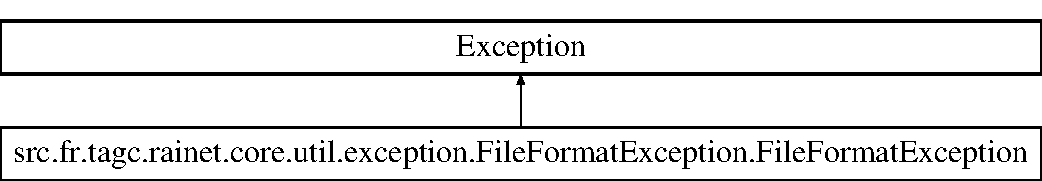
\includegraphics[height=2.000000cm]{classsrc_1_1fr_1_1tagc_1_1rainet_1_1core_1_1util_1_1exception_1_1FileFormatException_1_1FileFormatException}
\end{center}
\end{figure}
\subsection*{Public Member Functions}
\begin{DoxyCompactItemize}
\item 
\hypertarget{classsrc_1_1fr_1_1tagc_1_1rainet_1_1core_1_1util_1_1exception_1_1FileFormatException_1_1FileFormatException_a374b2a767ff7e33a4a67a6a751d29728}{}def {\bfseries \+\_\+\+\_\+init\+\_\+\+\_\+} (self, message)\label{classsrc_1_1fr_1_1tagc_1_1rainet_1_1core_1_1util_1_1exception_1_1FileFormatException_1_1FileFormatException_a374b2a767ff7e33a4a67a6a751d29728}

\item 
\hypertarget{classsrc_1_1fr_1_1tagc_1_1rainet_1_1core_1_1util_1_1exception_1_1FileFormatException_1_1FileFormatException_a6f6abefd1172772bc5c3909c596f4758}{}def {\bfseries print\+\_\+error} (self)\label{classsrc_1_1fr_1_1tagc_1_1rainet_1_1core_1_1util_1_1exception_1_1FileFormatException_1_1FileFormatException_a6f6abefd1172772bc5c3909c596f4758}

\end{DoxyCompactItemize}
\subsection*{Public Attributes}
\begin{DoxyCompactItemize}
\item 
\hypertarget{classsrc_1_1fr_1_1tagc_1_1rainet_1_1core_1_1util_1_1exception_1_1FileFormatException_1_1FileFormatException_aa199dfd8c7e58f6832074ee235628f21}{}{\bfseries message}\label{classsrc_1_1fr_1_1tagc_1_1rainet_1_1core_1_1util_1_1exception_1_1FileFormatException_1_1FileFormatException_aa199dfd8c7e58f6832074ee235628f21}

\end{DoxyCompactItemize}


\subsection{Detailed Description}
Exception raised in case of file format given in a method is not appropriated. 

The documentation for this class was generated from the following file\+:\begin{DoxyCompactItemize}
\item 
src/fr/tagc/rainet/core/util/exception/File\+Format\+Exception.\+py\end{DoxyCompactItemize}

\hypertarget{classsrc_1_1fr_1_1tagc_1_1rainet_1_1core_1_1util_1_1file_1_1FileUtils_1_1FileUtils}{}\section{src.\+fr.\+tagc.\+rainet.\+core.\+util.\+file.\+File\+Utils.\+File\+Utils Class Reference}
\label{classsrc_1_1fr_1_1tagc_1_1rainet_1_1core_1_1util_1_1file_1_1FileUtils_1_1FileUtils}\index{src.\+fr.\+tagc.\+rainet.\+core.\+util.\+file.\+File\+Utils.\+File\+Utils@{src.\+fr.\+tagc.\+rainet.\+core.\+util.\+file.\+File\+Utils.\+File\+Utils}}


This class contains static methods that are used to manipulate files like open  and close, but some others like find extension.  


Inheritance diagram for src.\+fr.\+tagc.\+rainet.\+core.\+util.\+file.\+File\+Utils.\+File\+Utils\+:\begin{figure}[H]
\begin{center}
\leavevmode
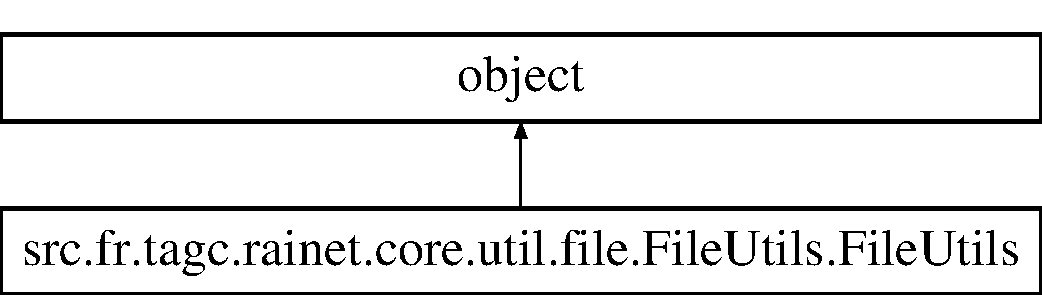
\includegraphics[height=2.000000cm]{classsrc_1_1fr_1_1tagc_1_1rainet_1_1core_1_1util_1_1file_1_1FileUtils_1_1FileUtils}
\end{center}
\end{figure}
\subsection*{Static Public Member Functions}
\begin{DoxyCompactItemize}
\item 
\hypertarget{classsrc_1_1fr_1_1tagc_1_1rainet_1_1core_1_1util_1_1file_1_1FileUtils_1_1FileUtils_a1ad81b043ababe6f08c5af6eb7a31641}{}def {\bfseries open\+\_\+text\+\_\+r} (path)\label{classsrc_1_1fr_1_1tagc_1_1rainet_1_1core_1_1util_1_1file_1_1FileUtils_1_1FileUtils_a1ad81b043ababe6f08c5af6eb7a31641}

\item 
\hypertarget{classsrc_1_1fr_1_1tagc_1_1rainet_1_1core_1_1util_1_1file_1_1FileUtils_1_1FileUtils_ac5142dd1a95af1d3ec203aa341492dd4}{}def {\bfseries open\+\_\+text\+\_\+w} (path)\label{classsrc_1_1fr_1_1tagc_1_1rainet_1_1core_1_1util_1_1file_1_1FileUtils_1_1FileUtils_ac5142dd1a95af1d3ec203aa341492dd4}

\item 
\hypertarget{classsrc_1_1fr_1_1tagc_1_1rainet_1_1core_1_1util_1_1file_1_1FileUtils_1_1FileUtils_abccf9b5e787cb9762babba235810b432}{}def {\bfseries check\+\_\+extension} (path)\label{classsrc_1_1fr_1_1tagc_1_1rainet_1_1core_1_1util_1_1file_1_1FileUtils_1_1FileUtils_abccf9b5e787cb9762babba235810b432}

\end{DoxyCompactItemize}


\subsection{Detailed Description}
This class contains static methods that are used to manipulate files like open  and close, but some others like find extension. 

  

The documentation for this class was generated from the following file\+:\begin{DoxyCompactItemize}
\item 
src/fr/tagc/rainet/core/util/file/File\+Utils.\+py\end{DoxyCompactItemize}

\hypertarget{classsrc_1_1fr_1_1tagc_1_1rainet_1_1core_1_1util_1_1log_1_1Logger_1_1Logger}{}\section{src.\+fr.\+tagc.\+rainet.\+core.\+util.\+log.\+Logger.\+Logger Class Reference}
\label{classsrc_1_1fr_1_1tagc_1_1rainet_1_1core_1_1util_1_1log_1_1Logger_1_1Logger}\index{src.\+fr.\+tagc.\+rainet.\+core.\+util.\+log.\+Logger.\+Logger@{src.\+fr.\+tagc.\+rainet.\+core.\+util.\+log.\+Logger.\+Logger}}


This class is a singleton used to manage logging It contains several method to add log at different level and manage both output to file and standard output.  


Inheritance diagram for src.\+fr.\+tagc.\+rainet.\+core.\+util.\+log.\+Logger.\+Logger\+:\begin{figure}[H]
\begin{center}
\leavevmode
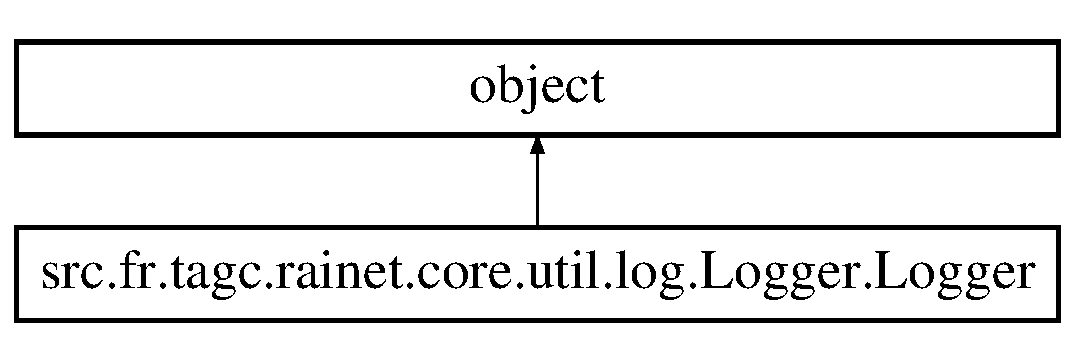
\includegraphics[height=2.000000cm]{classsrc_1_1fr_1_1tagc_1_1rainet_1_1core_1_1util_1_1log_1_1Logger_1_1Logger}
\end{center}
\end{figure}
\subsection*{Public Member Functions}
\begin{DoxyCompactItemize}
\item 
\hypertarget{classsrc_1_1fr_1_1tagc_1_1rainet_1_1core_1_1util_1_1log_1_1Logger_1_1Logger_a8b8db38c1df07ebf8eda30acc9213f04}{}def {\bfseries \+\_\+\+\_\+init\+\_\+\+\_\+} (self)\label{classsrc_1_1fr_1_1tagc_1_1rainet_1_1core_1_1util_1_1log_1_1Logger_1_1Logger_a8b8db38c1df07ebf8eda30acc9213f04}

\item 
\hypertarget{classsrc_1_1fr_1_1tagc_1_1rainet_1_1core_1_1util_1_1log_1_1Logger_1_1Logger_ab5fbcdb8ad161e3e9f1dad276824839c}{}def {\bfseries info} (self, message)\label{classsrc_1_1fr_1_1tagc_1_1rainet_1_1core_1_1util_1_1log_1_1Logger_1_1Logger_ab5fbcdb8ad161e3e9f1dad276824839c}

\item 
\hypertarget{classsrc_1_1fr_1_1tagc_1_1rainet_1_1core_1_1util_1_1log_1_1Logger_1_1Logger_a228c6106085b1ff88bd9c6f20c95e39e}{}def {\bfseries warning} (self, message)\label{classsrc_1_1fr_1_1tagc_1_1rainet_1_1core_1_1util_1_1log_1_1Logger_1_1Logger_a228c6106085b1ff88bd9c6f20c95e39e}

\item 
\hypertarget{classsrc_1_1fr_1_1tagc_1_1rainet_1_1core_1_1util_1_1log_1_1Logger_1_1Logger_a6181f643c1339d15b154c4c8ec3ec86f}{}def {\bfseries error} (self, message)\label{classsrc_1_1fr_1_1tagc_1_1rainet_1_1core_1_1util_1_1log_1_1Logger_1_1Logger_a6181f643c1339d15b154c4c8ec3ec86f}

\item 
\hypertarget{classsrc_1_1fr_1_1tagc_1_1rainet_1_1core_1_1util_1_1log_1_1Logger_1_1Logger_a01b79ca66c78f7c42a8145636595fb34}{}def {\bfseries critical} (self, message)\label{classsrc_1_1fr_1_1tagc_1_1rainet_1_1core_1_1util_1_1log_1_1Logger_1_1Logger_a01b79ca66c78f7c42a8145636595fb34}

\end{DoxyCompactItemize}
\subsection*{Static Public Member Functions}
\begin{DoxyCompactItemize}
\item 
\hypertarget{classsrc_1_1fr_1_1tagc_1_1rainet_1_1core_1_1util_1_1log_1_1Logger_1_1Logger_a8264bb686116fcde3fafac8872915a7d}{}def {\bfseries set\+Logger} ()\label{classsrc_1_1fr_1_1tagc_1_1rainet_1_1core_1_1util_1_1log_1_1Logger_1_1Logger_a8264bb686116fcde3fafac8872915a7d}

\item 
\hypertarget{classsrc_1_1fr_1_1tagc_1_1rainet_1_1core_1_1util_1_1log_1_1Logger_1_1Logger_a07abf08bb9643f57feeba282895f5b1b}{}def {\bfseries get\+\_\+instance} ()\label{classsrc_1_1fr_1_1tagc_1_1rainet_1_1core_1_1util_1_1log_1_1Logger_1_1Logger_a07abf08bb9643f57feeba282895f5b1b}

\end{DoxyCompactItemize}
\subsection*{Public Attributes}
\begin{DoxyCompactItemize}
\item 
\hypertarget{classsrc_1_1fr_1_1tagc_1_1rainet_1_1core_1_1util_1_1log_1_1Logger_1_1Logger_a4602026d1e48039f2ba504e357c095aa}{}{\bfseries logg}\label{classsrc_1_1fr_1_1tagc_1_1rainet_1_1core_1_1util_1_1log_1_1Logger_1_1Logger_a4602026d1e48039f2ba504e357c095aa}

\end{DoxyCompactItemize}


\subsection{Detailed Description}
This class is a singleton used to manage logging It contains several method to add log at different level and manage both output to file and standard output. 

The documentation for this class was generated from the following file\+:\begin{DoxyCompactItemize}
\item 
src/fr/tagc/rainet/core/util/log/Logger.\+py\end{DoxyCompactItemize}

\hypertarget{classsrc_1_1fr_1_1tagc_1_1rainet_1_1core_1_1data_1_1Protein_1_1Protein}{}\section{src.\+fr.\+tagc.\+rainet.\+core.\+data.\+Protein.\+Protein Class Reference}
\label{classsrc_1_1fr_1_1tagc_1_1rainet_1_1core_1_1data_1_1Protein_1_1Protein}\index{src.\+fr.\+tagc.\+rainet.\+core.\+data.\+Protein.\+Protein@{src.\+fr.\+tagc.\+rainet.\+core.\+data.\+Protein.\+Protein}}


This class describe a protein obtained from query on the Uniprot D\+B.  


Inheritance diagram for src.\+fr.\+tagc.\+rainet.\+core.\+data.\+Protein.\+Protein\+:\begin{figure}[H]
\begin{center}
\leavevmode
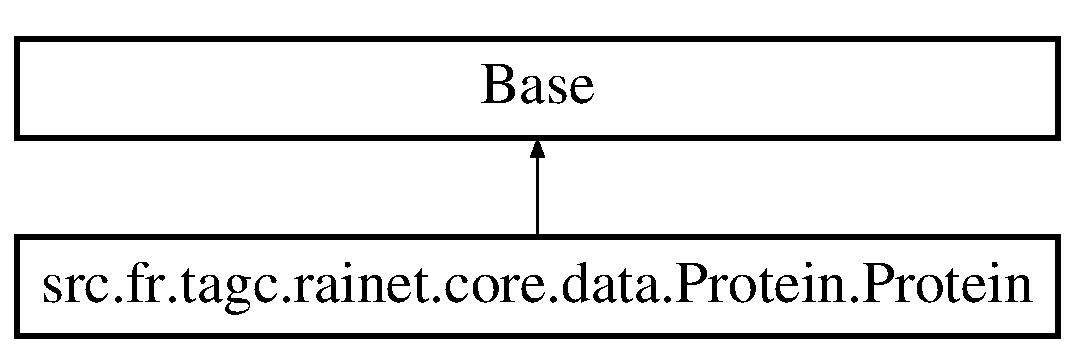
\includegraphics[height=2.000000cm]{classsrc_1_1fr_1_1tagc_1_1rainet_1_1core_1_1data_1_1Protein_1_1Protein}
\end{center}
\end{figure}
\subsection*{Public Member Functions}
\begin{DoxyCompactItemize}
\item 
def \hyperlink{classsrc_1_1fr_1_1tagc_1_1rainet_1_1core_1_1data_1_1Protein_1_1Protein_a2ef26c34c2c219ed62056ac37cc540cb}{\+\_\+\+\_\+init\+\_\+\+\_\+} (self, prot\+\_\+ac, prot\+\_\+id, prot\+\_\+name, prot\+\_\+symbol, prot\+\_\+synonym, prot\+\_\+organism, prot\+\_\+length, prot\+\_\+fragment)
\begin{DoxyCompactList}\small\item\em The \hyperlink{classsrc_1_1fr_1_1tagc_1_1rainet_1_1core_1_1data_1_1Protein_1_1Protein}{Protein} constructor. \end{DoxyCompactList}\item 
\hypertarget{classsrc_1_1fr_1_1tagc_1_1rainet_1_1core_1_1data_1_1Protein_1_1Protein_a388c7e4636cc5726d58b1415e96786b4}{}def \hyperlink{classsrc_1_1fr_1_1tagc_1_1rainet_1_1core_1_1data_1_1Protein_1_1Protein_a388c7e4636cc5726d58b1415e96786b4}{add\+\_\+to\+\_\+session} (self)\label{classsrc_1_1fr_1_1tagc_1_1rainet_1_1core_1_1data_1_1Protein_1_1Protein_a388c7e4636cc5726d58b1415e96786b4}

\begin{DoxyCompactList}\small\item\em Add the object to S\+Q\+L\+Alchemy session. \end{DoxyCompactList}\end{DoxyCompactItemize}
\subsection*{Public Attributes}
\begin{DoxyCompactItemize}
\item 
\hypertarget{classsrc_1_1fr_1_1tagc_1_1rainet_1_1core_1_1data_1_1Protein_1_1Protein_a60ff9506c688577c0ddd8bcdb7a9466f}{}{\bfseries uniprot\+A\+C}\label{classsrc_1_1fr_1_1tagc_1_1rainet_1_1core_1_1data_1_1Protein_1_1Protein_a60ff9506c688577c0ddd8bcdb7a9466f}

\item 
\hypertarget{classsrc_1_1fr_1_1tagc_1_1rainet_1_1core_1_1data_1_1Protein_1_1Protein_a3bdaf8cefac00e143a6257a66c29ef17}{}{\bfseries uniprot\+I\+D}\label{classsrc_1_1fr_1_1tagc_1_1rainet_1_1core_1_1data_1_1Protein_1_1Protein_a3bdaf8cefac00e143a6257a66c29ef17}

\item 
\hypertarget{classsrc_1_1fr_1_1tagc_1_1rainet_1_1core_1_1data_1_1Protein_1_1Protein_a0054b41ccd6ec6039a1404ef21d066b6}{}{\bfseries uniprot\+Name}\label{classsrc_1_1fr_1_1tagc_1_1rainet_1_1core_1_1data_1_1Protein_1_1Protein_a0054b41ccd6ec6039a1404ef21d066b6}

\item 
\hypertarget{classsrc_1_1fr_1_1tagc_1_1rainet_1_1core_1_1data_1_1Protein_1_1Protein_ad8f435c514b79080683e30a9c581145e}{}{\bfseries uniprot\+Gene\+Symbol}\label{classsrc_1_1fr_1_1tagc_1_1rainet_1_1core_1_1data_1_1Protein_1_1Protein_ad8f435c514b79080683e30a9c581145e}

\item 
\hypertarget{classsrc_1_1fr_1_1tagc_1_1rainet_1_1core_1_1data_1_1Protein_1_1Protein_a3c122b230551a29d5f2f0a1d55953589}{}{\bfseries organism}\label{classsrc_1_1fr_1_1tagc_1_1rainet_1_1core_1_1data_1_1Protein_1_1Protein_a3c122b230551a29d5f2f0a1d55953589}

\item 
\hypertarget{classsrc_1_1fr_1_1tagc_1_1rainet_1_1core_1_1data_1_1Protein_1_1Protein_aef44a8df4a1fdc4f12addd6955644866}{}{\bfseries protein\+Length}\label{classsrc_1_1fr_1_1tagc_1_1rainet_1_1core_1_1data_1_1Protein_1_1Protein_aef44a8df4a1fdc4f12addd6955644866}

\item 
\hypertarget{classsrc_1_1fr_1_1tagc_1_1rainet_1_1core_1_1data_1_1Protein_1_1Protein_a39165a3c9fa3f829cfa1c1f87fb178c3}{}{\bfseries id\+Fragment}\label{classsrc_1_1fr_1_1tagc_1_1rainet_1_1core_1_1data_1_1Protein_1_1Protein_a39165a3c9fa3f829cfa1c1f87fb178c3}

\item 
\hypertarget{classsrc_1_1fr_1_1tagc_1_1rainet_1_1core_1_1data_1_1Protein_1_1Protein_a7004a85c545f20515a29a0b19f51387a}{}{\bfseries uniprot\+Synonym\+Gene\+Symbols}\label{classsrc_1_1fr_1_1tagc_1_1rainet_1_1core_1_1data_1_1Protein_1_1Protein_a7004a85c545f20515a29a0b19f51387a}

\end{DoxyCompactItemize}
\subsection*{Static Public Attributes}
\begin{DoxyCompactItemize}
\item 
\hypertarget{classsrc_1_1fr_1_1tagc_1_1rainet_1_1core_1_1data_1_1Protein_1_1Protein_a2798db19d4f935c15a4effa12decd9ef}{}tuple {\bfseries uniprot\+A\+C} = Column( String, primary\+\_\+key = True )\label{classsrc_1_1fr_1_1tagc_1_1rainet_1_1core_1_1data_1_1Protein_1_1Protein_a2798db19d4f935c15a4effa12decd9ef}

\item 
\hypertarget{classsrc_1_1fr_1_1tagc_1_1rainet_1_1core_1_1data_1_1Protein_1_1Protein_a6857fd877f8bc86e5785a7a401938377}{}tuple {\bfseries uniprot\+I\+D} = Column( String )\label{classsrc_1_1fr_1_1tagc_1_1rainet_1_1core_1_1data_1_1Protein_1_1Protein_a6857fd877f8bc86e5785a7a401938377}

\item 
\hypertarget{classsrc_1_1fr_1_1tagc_1_1rainet_1_1core_1_1data_1_1Protein_1_1Protein_a61c9e7352642849c9a3af1b462758bea}{}tuple {\bfseries uniprot\+Name} = Column( String )\label{classsrc_1_1fr_1_1tagc_1_1rainet_1_1core_1_1data_1_1Protein_1_1Protein_a61c9e7352642849c9a3af1b462758bea}

\item 
\hypertarget{classsrc_1_1fr_1_1tagc_1_1rainet_1_1core_1_1data_1_1Protein_1_1Protein_a33c562adba937c1992b1fa1fdcfc2f74}{}tuple {\bfseries uniprot\+Gene\+Symbol} = Column( String )\label{classsrc_1_1fr_1_1tagc_1_1rainet_1_1core_1_1data_1_1Protein_1_1Protein_a33c562adba937c1992b1fa1fdcfc2f74}

\item 
\hypertarget{classsrc_1_1fr_1_1tagc_1_1rainet_1_1core_1_1data_1_1Protein_1_1Protein_a1fc531019a865d0542a703f7451f7ce9}{}tuple {\bfseries organism} = Column( String )\label{classsrc_1_1fr_1_1tagc_1_1rainet_1_1core_1_1data_1_1Protein_1_1Protein_a1fc531019a865d0542a703f7451f7ce9}

\item 
\hypertarget{classsrc_1_1fr_1_1tagc_1_1rainet_1_1core_1_1data_1_1Protein_1_1Protein_afb1a9297547302bb073f3d13c41dd335}{}tuple {\bfseries protein\+Length} = Column( Integer )\label{classsrc_1_1fr_1_1tagc_1_1rainet_1_1core_1_1data_1_1Protein_1_1Protein_afb1a9297547302bb073f3d13c41dd335}

\item 
\hypertarget{classsrc_1_1fr_1_1tagc_1_1rainet_1_1core_1_1data_1_1Protein_1_1Protein_ae59a8d90168f71b0b3cc00132bca8fe2}{}tuple {\bfseries id\+Fragment} = Column( Boolean )\label{classsrc_1_1fr_1_1tagc_1_1rainet_1_1core_1_1data_1_1Protein_1_1Protein_ae59a8d90168f71b0b3cc00132bca8fe2}

\item 
\hypertarget{classsrc_1_1fr_1_1tagc_1_1rainet_1_1core_1_1data_1_1Protein_1_1Protein_ade8cb49011448d5bac8b6b82c40166f8}{}tuple {\bfseries uniprot\+Synonym\+Gene\+Symbols} = relationship(\textquotesingle{}Synonym\+Gene\+Symbol\textquotesingle{}, backref=\textquotesingle{}protein\textquotesingle{})\label{classsrc_1_1fr_1_1tagc_1_1rainet_1_1core_1_1data_1_1Protein_1_1Protein_ade8cb49011448d5bac8b6b82c40166f8}

\end{DoxyCompactItemize}


\subsection{Detailed Description}
This class describe a protein obtained from query on the Uniprot D\+B. 

this class has a one-\/to-\/many relationship with the class Synonym\+Gene\+Symbol 

\subsection{Constructor \& Destructor Documentation}
\hypertarget{classsrc_1_1fr_1_1tagc_1_1rainet_1_1core_1_1data_1_1Protein_1_1Protein_a2ef26c34c2c219ed62056ac37cc540cb}{}\index{src\+::fr\+::tagc\+::rainet\+::core\+::data\+::\+Protein\+::\+Protein@{src\+::fr\+::tagc\+::rainet\+::core\+::data\+::\+Protein\+::\+Protein}!\+\_\+\+\_\+init\+\_\+\+\_\+@{\+\_\+\+\_\+init\+\_\+\+\_\+}}
\index{\+\_\+\+\_\+init\+\_\+\+\_\+@{\+\_\+\+\_\+init\+\_\+\+\_\+}!src\+::fr\+::tagc\+::rainet\+::core\+::data\+::\+Protein\+::\+Protein@{src\+::fr\+::tagc\+::rainet\+::core\+::data\+::\+Protein\+::\+Protein}}
\subsubsection[{\+\_\+\+\_\+init\+\_\+\+\_\+}]{\setlength{\rightskip}{0pt plus 5cm}def src.\+fr.\+tagc.\+rainet.\+core.\+data.\+Protein.\+Protein.\+\_\+\+\_\+init\+\_\+\+\_\+ (
\begin{DoxyParamCaption}
\item[{}]{self, }
\item[{}]{prot\+\_\+ac, }
\item[{}]{prot\+\_\+id, }
\item[{}]{prot\+\_\+name, }
\item[{}]{prot\+\_\+symbol, }
\item[{}]{prot\+\_\+synonym, }
\item[{}]{prot\+\_\+organism, }
\item[{}]{prot\+\_\+length, }
\item[{}]{prot\+\_\+fragment}
\end{DoxyParamCaption}
)}\label{classsrc_1_1fr_1_1tagc_1_1rainet_1_1core_1_1data_1_1Protein_1_1Protein_a2ef26c34c2c219ed62056ac37cc540cb}


The \hyperlink{classsrc_1_1fr_1_1tagc_1_1rainet_1_1core_1_1data_1_1Protein_1_1Protein}{Protein} constructor. 


\begin{DoxyParams}{Parameters}
{\em prot\+\_\+ac} & \+: string -\/ The Uniprot accession number of the protein \\
\hline
{\em prot\+\_\+id} & \+: string -\/ The Uniprot I\+D of the protein \\
\hline
{\em prot\+\_\+name} & \+: string -\/ The Uniprot I\+D of the protein \\
\hline
{\em prot\+\_\+symbol} & \+: string -\/ The Uniprot gene symbol of the protein \\
\hline
{\em prot\+\_\+synonym} & \+: string -\/ The list of Uniprot gene symbol synonyms of the protein \\
\hline
{\em prot\+\_\+organism} & \+: string -\/ The organism of the protein \\
\hline
{\em prot\+\_\+length} & \+: string -\/ The length of protein \\
\hline
{\em prot\+\_\+fragment} & \+: boolean -\/ \\
\hline
\end{DoxyParams}


The documentation for this class was generated from the following file\+:\begin{DoxyCompactItemize}
\item 
src/fr/tagc/rainet/core/data/Protein.\+py\end{DoxyCompactItemize}

\hypertarget{classsrc_1_1fr_1_1tagc_1_1rainet_1_1core_1_1Rainet_1_1Rainet}{}\section{src.\+fr.\+tagc.\+rainet.\+core.\+Rainet.\+Rainet Class Reference}
\label{classsrc_1_1fr_1_1tagc_1_1rainet_1_1core_1_1Rainet_1_1Rainet}\index{src.\+fr.\+tagc.\+rainet.\+core.\+Rainet.\+Rainet@{src.\+fr.\+tagc.\+rainet.\+core.\+Rainet.\+Rainet}}


This is the main class of the \hyperlink{classsrc_1_1fr_1_1tagc_1_1rainet_1_1core_1_1Rainet_1_1Rainet}{Rainet} project.  


Inheritance diagram for src.\+fr.\+tagc.\+rainet.\+core.\+Rainet.\+Rainet\+:\begin{figure}[H]
\begin{center}
\leavevmode
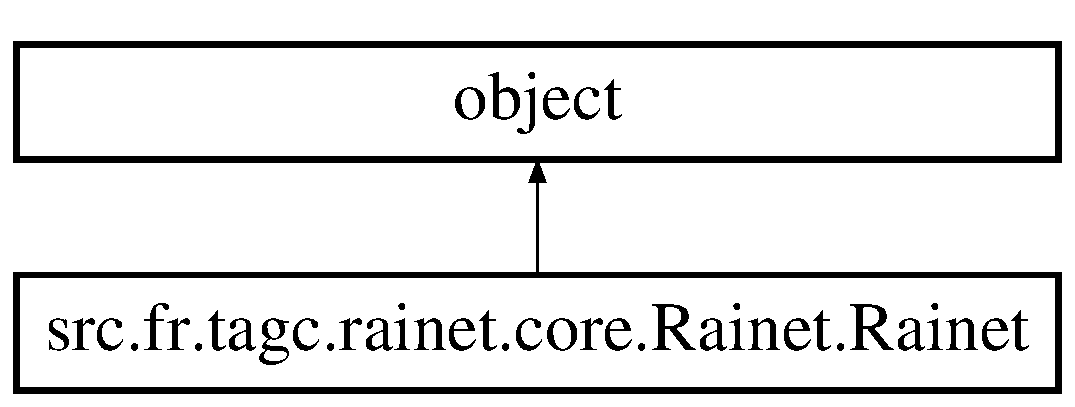
\includegraphics[height=2.000000cm]{classsrc_1_1fr_1_1tagc_1_1rainet_1_1core_1_1Rainet_1_1Rainet}
\end{center}
\end{figure}
\subsection*{Public Member Functions}
\begin{DoxyCompactItemize}
\item 
def \hyperlink{classsrc_1_1fr_1_1tagc_1_1rainet_1_1core_1_1Rainet_1_1Rainet_a92e1698d37d733e389aea584f74885f2}{\+\_\+\+\_\+init\+\_\+\+\_\+} (self, db\+\_\+path)
\begin{DoxyCompactList}\small\item\em Initialize the \hyperlink{classsrc_1_1fr_1_1tagc_1_1rainet_1_1core_1_1Rainet_1_1Rainet}{Rainet} object. \end{DoxyCompactList}\item 
\hypertarget{classsrc_1_1fr_1_1tagc_1_1rainet_1_1core_1_1Rainet_1_1Rainet_a21be49bba245c039044a96f40dfcc5de}{}def \hyperlink{classsrc_1_1fr_1_1tagc_1_1rainet_1_1core_1_1Rainet_1_1Rainet_a21be49bba245c039044a96f40dfcc5de}{insert\+\_\+data} (self)\label{classsrc_1_1fr_1_1tagc_1_1rainet_1_1core_1_1Rainet_1_1Rainet_a21be49bba245c039044a96f40dfcc5de}

\begin{DoxyCompactList}\small\item\em Insert the various data to the Database using file defined in the configuration file. \end{DoxyCompactList}\end{DoxyCompactItemize}
\subsection*{Public Attributes}
\begin{DoxyCompactItemize}
\item 
\hypertarget{classsrc_1_1fr_1_1tagc_1_1rainet_1_1core_1_1Rainet_1_1Rainet_a0a2a54eebfd211da5e522331af6bc143}{}{\bfseries D\+B\+Path}\label{classsrc_1_1fr_1_1tagc_1_1rainet_1_1core_1_1Rainet_1_1Rainet_a0a2a54eebfd211da5e522331af6bc143}

\end{DoxyCompactItemize}


\subsection{Detailed Description}
This is the main class of the \hyperlink{classsrc_1_1fr_1_1tagc_1_1rainet_1_1core_1_1Rainet_1_1Rainet}{Rainet} project. 

It contains methods used to insert data to the database and make several type of analysis 

\subsection{Constructor \& Destructor Documentation}
\hypertarget{classsrc_1_1fr_1_1tagc_1_1rainet_1_1core_1_1Rainet_1_1Rainet_a92e1698d37d733e389aea584f74885f2}{}\index{src\+::fr\+::tagc\+::rainet\+::core\+::\+Rainet\+::\+Rainet@{src\+::fr\+::tagc\+::rainet\+::core\+::\+Rainet\+::\+Rainet}!\+\_\+\+\_\+init\+\_\+\+\_\+@{\+\_\+\+\_\+init\+\_\+\+\_\+}}
\index{\+\_\+\+\_\+init\+\_\+\+\_\+@{\+\_\+\+\_\+init\+\_\+\+\_\+}!src\+::fr\+::tagc\+::rainet\+::core\+::\+Rainet\+::\+Rainet@{src\+::fr\+::tagc\+::rainet\+::core\+::\+Rainet\+::\+Rainet}}
\subsubsection[{\+\_\+\+\_\+init\+\_\+\+\_\+}]{\setlength{\rightskip}{0pt plus 5cm}def src.\+fr.\+tagc.\+rainet.\+core.\+Rainet.\+Rainet.\+\_\+\+\_\+init\+\_\+\+\_\+ (
\begin{DoxyParamCaption}
\item[{}]{self, }
\item[{}]{db\+\_\+path}
\end{DoxyParamCaption}
)}\label{classsrc_1_1fr_1_1tagc_1_1rainet_1_1core_1_1Rainet_1_1Rainet_a92e1698d37d733e389aea584f74885f2}


Initialize the \hyperlink{classsrc_1_1fr_1_1tagc_1_1rainet_1_1core_1_1Rainet_1_1Rainet}{Rainet} object. 


\begin{DoxyParams}{Parameters}
{\em db\+\_\+path} & \+: string -\/ The path to the database \\
\hline
\end{DoxyParams}


The documentation for this class was generated from the following file\+:\begin{DoxyCompactItemize}
\item 
src/fr/tagc/rainet/core/Rainet.\+py\end{DoxyCompactItemize}

\hypertarget{classsrc_1_1fr_1_1tagc_1_1rainet_1_1core_1_1util_1_1exception_1_1RainetException_1_1RainetException}{}\section{src.\+fr.\+tagc.\+rainet.\+core.\+util.\+exception.\+Rainet\+Exception.\+Rainet\+Exception Class Reference}
\label{classsrc_1_1fr_1_1tagc_1_1rainet_1_1core_1_1util_1_1exception_1_1RainetException_1_1RainetException}\index{src.\+fr.\+tagc.\+rainet.\+core.\+util.\+exception.\+Rainet\+Exception.\+Rainet\+Exception@{src.\+fr.\+tagc.\+rainet.\+core.\+util.\+exception.\+Rainet\+Exception.\+Rainet\+Exception}}


Generic exception used to identify catched and raised exceptions and errors from Rainet code.  


Inheritance diagram for src.\+fr.\+tagc.\+rainet.\+core.\+util.\+exception.\+Rainet\+Exception.\+Rainet\+Exception\+:\begin{figure}[H]
\begin{center}
\leavevmode
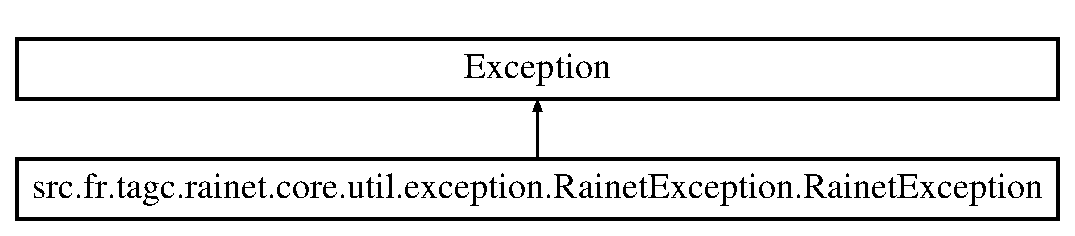
\includegraphics[height=2.000000cm]{classsrc_1_1fr_1_1tagc_1_1rainet_1_1core_1_1util_1_1exception_1_1RainetException_1_1RainetException}
\end{center}
\end{figure}
\subsection*{Public Member Functions}
\begin{DoxyCompactItemize}
\item 
def \hyperlink{classsrc_1_1fr_1_1tagc_1_1rainet_1_1core_1_1util_1_1exception_1_1RainetException_1_1RainetException_aacef80ab04c0067ea376b4dc436c3ba7}{\+\_\+\+\_\+init\+\_\+\+\_\+}
\begin{DoxyCompactList}\small\item\em Initialize the exception. \end{DoxyCompactList}\item 
\hypertarget{classsrc_1_1fr_1_1tagc_1_1rainet_1_1core_1_1util_1_1exception_1_1RainetException_1_1RainetException_a1c16b6658657b95368ad3c349f291be3}{}def \hyperlink{classsrc_1_1fr_1_1tagc_1_1rainet_1_1core_1_1util_1_1exception_1_1RainetException_1_1RainetException_a1c16b6658657b95368ad3c349f291be3}{to\+\_\+string} (self)\label{classsrc_1_1fr_1_1tagc_1_1rainet_1_1core_1_1util_1_1exception_1_1RainetException_1_1RainetException_a1c16b6658657b95368ad3c349f291be3}

\begin{DoxyCompactList}\small\item\em Display the exception message and stack trace. \end{DoxyCompactList}\end{DoxyCompactItemize}
\subsection*{Public Attributes}
\begin{DoxyCompactItemize}
\item 
\hypertarget{classsrc_1_1fr_1_1tagc_1_1rainet_1_1core_1_1util_1_1exception_1_1RainetException_1_1RainetException_aa81e62532f4f9814b3ce1c6f9aca028f}{}{\bfseries exception}\label{classsrc_1_1fr_1_1tagc_1_1rainet_1_1core_1_1util_1_1exception_1_1RainetException_1_1RainetException_aa81e62532f4f9814b3ce1c6f9aca028f}

\item 
\hypertarget{classsrc_1_1fr_1_1tagc_1_1rainet_1_1core_1_1util_1_1exception_1_1RainetException_1_1RainetException_a31c58d9d925221fd6499dfc8fe0e2609}{}{\bfseries message}\label{classsrc_1_1fr_1_1tagc_1_1rainet_1_1core_1_1util_1_1exception_1_1RainetException_1_1RainetException_a31c58d9d925221fd6499dfc8fe0e2609}

\end{DoxyCompactItemize}


\subsection{Detailed Description}
Generic exception used to identify catched and raised exceptions and errors from Rainet code. 

\subsection{Constructor \& Destructor Documentation}
\hypertarget{classsrc_1_1fr_1_1tagc_1_1rainet_1_1core_1_1util_1_1exception_1_1RainetException_1_1RainetException_aacef80ab04c0067ea376b4dc436c3ba7}{}\index{src\+::fr\+::tagc\+::rainet\+::core\+::util\+::exception\+::\+Rainet\+Exception\+::\+Rainet\+Exception@{src\+::fr\+::tagc\+::rainet\+::core\+::util\+::exception\+::\+Rainet\+Exception\+::\+Rainet\+Exception}!\+\_\+\+\_\+init\+\_\+\+\_\+@{\+\_\+\+\_\+init\+\_\+\+\_\+}}
\index{\+\_\+\+\_\+init\+\_\+\+\_\+@{\+\_\+\+\_\+init\+\_\+\+\_\+}!src\+::fr\+::tagc\+::rainet\+::core\+::util\+::exception\+::\+Rainet\+Exception\+::\+Rainet\+Exception@{src\+::fr\+::tagc\+::rainet\+::core\+::util\+::exception\+::\+Rainet\+Exception\+::\+Rainet\+Exception}}
\subsubsection[{\+\_\+\+\_\+init\+\_\+\+\_\+}]{\setlength{\rightskip}{0pt plus 5cm}def src.\+fr.\+tagc.\+rainet.\+core.\+util.\+exception.\+Rainet\+Exception.\+Rainet\+Exception.\+\_\+\+\_\+init\+\_\+\+\_\+ (
\begin{DoxyParamCaption}
\item[{}]{self, }
\item[{}]{mess, }
\item[{}]{excep = {\ttfamily None}}
\end{DoxyParamCaption}
)}\label{classsrc_1_1fr_1_1tagc_1_1rainet_1_1core_1_1util_1_1exception_1_1RainetException_1_1RainetException_aacef80ab04c0067ea376b4dc436c3ba7}


Initialize the exception. 


\begin{DoxyParams}{Parameters}
{\em mess} & \+: string -\/ The message associated to the exception \\
\hline
{\em excep} & \+: Exception -\/ The Exception associated to the exception (optional) \\
\hline
\end{DoxyParams}


The documentation for this class was generated from the following file\+:\begin{DoxyCompactItemize}
\item 
src/fr/tagc/rainet/core/util/exception/Rainet\+Exception.\+py\end{DoxyCompactItemize}

\hypertarget{classsrc_1_1fr_1_1tagc_1_1rainet_1_1core_1_1util_1_1sql_1_1SQLAlchemyUtil_1_1SQLAlchemyUtil}{}\section{src.\+fr.\+tagc.\+rainet.\+core.\+util.\+sql.\+S\+Q\+L\+Alchemy\+Util.\+S\+Q\+L\+Alchemy\+Util Class Reference}
\label{classsrc_1_1fr_1_1tagc_1_1rainet_1_1core_1_1util_1_1sql_1_1SQLAlchemyUtil_1_1SQLAlchemyUtil}\index{src.\+fr.\+tagc.\+rainet.\+core.\+util.\+sql.\+S\+Q\+L\+Alchemy\+Util.\+S\+Q\+L\+Alchemy\+Util@{src.\+fr.\+tagc.\+rainet.\+core.\+util.\+sql.\+S\+Q\+L\+Alchemy\+Util.\+S\+Q\+L\+Alchemy\+Util}}


this class contains static methods aiming to simplify the usage of S\+Q\+Lalchemy results of query  


Inheritance diagram for src.\+fr.\+tagc.\+rainet.\+core.\+util.\+sql.\+S\+Q\+L\+Alchemy\+Util.\+S\+Q\+L\+Alchemy\+Util\+:\begin{figure}[H]
\begin{center}
\leavevmode
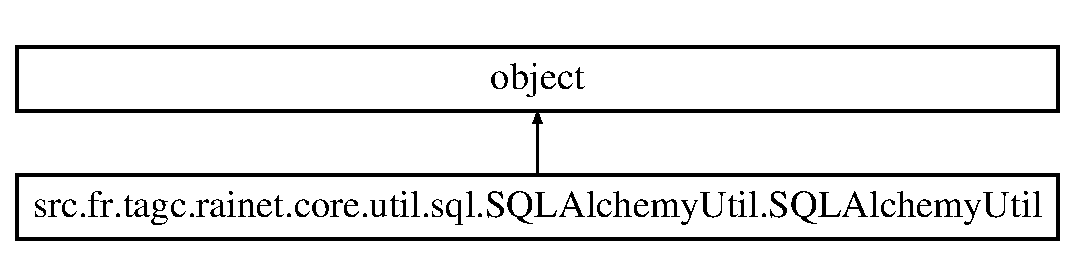
\includegraphics[height=2.000000cm]{classsrc_1_1fr_1_1tagc_1_1rainet_1_1core_1_1util_1_1sql_1_1SQLAlchemyUtil_1_1SQLAlchemyUtil}
\end{center}
\end{figure}
\subsection*{Static Public Member Functions}
\begin{DoxyCompactItemize}
\item 
\hypertarget{classsrc_1_1fr_1_1tagc_1_1rainet_1_1core_1_1util_1_1sql_1_1SQLAlchemyUtil_1_1SQLAlchemyUtil_a102b42a21b6a74a46f7cf150ac3c8e2c}{}def {\bfseries format\+\_\+list\+\_\+column} (sql\+\_\+alchemy\+\_\+list)\label{classsrc_1_1fr_1_1tagc_1_1rainet_1_1core_1_1util_1_1sql_1_1SQLAlchemyUtil_1_1SQLAlchemyUtil_a102b42a21b6a74a46f7cf150ac3c8e2c}

\item 
\hypertarget{classsrc_1_1fr_1_1tagc_1_1rainet_1_1core_1_1util_1_1sql_1_1SQLAlchemyUtil_1_1SQLAlchemyUtil_a5d8c69d5c129773169fd4b754b6c4243}{}def {\bfseries format\+\_\+list\+\_\+object} (sql\+\_\+alchemy\+\_\+list)\label{classsrc_1_1fr_1_1tagc_1_1rainet_1_1core_1_1util_1_1sql_1_1SQLAlchemyUtil_1_1SQLAlchemyUtil_a5d8c69d5c129773169fd4b754b6c4243}

\end{DoxyCompactItemize}


\subsection{Detailed Description}
this class contains static methods aiming to simplify the usage of S\+Q\+Lalchemy results of query 

The documentation for this class was generated from the following file\+:\begin{DoxyCompactItemize}
\item 
src/fr/tagc/rainet/core/util/sql/S\+Q\+L\+Alchemy\+Util.\+py\end{DoxyCompactItemize}

\hypertarget{classsrc_1_1fr_1_1tagc_1_1rainet_1_1core_1_1util_1_1sql_1_1SQLManager_1_1SQLManager}{}\section{src.\+fr.\+tagc.\+rainet.\+core.\+util.\+sql.\+S\+Q\+L\+Manager.\+S\+Q\+L\+Manager Class Reference}
\label{classsrc_1_1fr_1_1tagc_1_1rainet_1_1core_1_1util_1_1sql_1_1SQLManager_1_1SQLManager}\index{src.\+fr.\+tagc.\+rainet.\+core.\+util.\+sql.\+S\+Q\+L\+Manager.\+S\+Q\+L\+Manager@{src.\+fr.\+tagc.\+rainet.\+core.\+util.\+sql.\+S\+Q\+L\+Manager.\+S\+Q\+L\+Manager}}


This class is a singleton aiming to manage S\+Q\+L connection to the database The singleton is able to manage the creation of a S\+Q\+L\+Alchemy Session to the database it has been initiated with.  


Inheritance diagram for src.\+fr.\+tagc.\+rainet.\+core.\+util.\+sql.\+S\+Q\+L\+Manager.\+S\+Q\+L\+Manager\+:\begin{figure}[H]
\begin{center}
\leavevmode
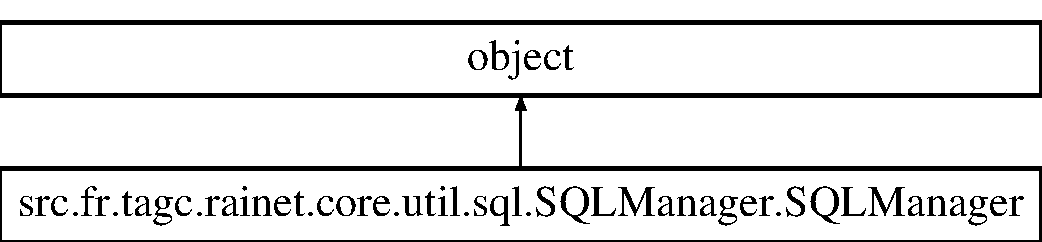
\includegraphics[height=2.000000cm]{classsrc_1_1fr_1_1tagc_1_1rainet_1_1core_1_1util_1_1sql_1_1SQLManager_1_1SQLManager}
\end{center}
\end{figure}
\subsection*{Public Member Functions}
\begin{DoxyCompactItemize}
\item 
\hypertarget{classsrc_1_1fr_1_1tagc_1_1rainet_1_1core_1_1util_1_1sql_1_1SQLManager_1_1SQLManager_a8e883e3a2d50c570379a36e533f435c8}{}def {\bfseries \+\_\+\+\_\+init\+\_\+\+\_\+} (self)\label{classsrc_1_1fr_1_1tagc_1_1rainet_1_1core_1_1util_1_1sql_1_1SQLManager_1_1SQLManager_a8e883e3a2d50c570379a36e533f435c8}

\item 
\hypertarget{classsrc_1_1fr_1_1tagc_1_1rainet_1_1core_1_1util_1_1sql_1_1SQLManager_1_1SQLManager_ade8c70005119df93c018383736dad4c5}{}def {\bfseries get\+\_\+session} (self)\label{classsrc_1_1fr_1_1tagc_1_1rainet_1_1core_1_1util_1_1sql_1_1SQLManager_1_1SQLManager_ade8c70005119df93c018383736dad4c5}

\item 
\hypertarget{classsrc_1_1fr_1_1tagc_1_1rainet_1_1core_1_1util_1_1sql_1_1SQLManager_1_1SQLManager_ae4f79e502aee77fc01175a22e284e322}{}def {\bfseries close\+\_\+session} (self)\label{classsrc_1_1fr_1_1tagc_1_1rainet_1_1core_1_1util_1_1sql_1_1SQLManager_1_1SQLManager_ae4f79e502aee77fc01175a22e284e322}

\item 
\hypertarget{classsrc_1_1fr_1_1tagc_1_1rainet_1_1core_1_1util_1_1sql_1_1SQLManager_1_1SQLManager_af1703b4d26840eea064d95763d21a212}{}def {\bfseries commit} (self)\label{classsrc_1_1fr_1_1tagc_1_1rainet_1_1core_1_1util_1_1sql_1_1SQLManager_1_1SQLManager_af1703b4d26840eea064d95763d21a212}

\item 
\hypertarget{classsrc_1_1fr_1_1tagc_1_1rainet_1_1core_1_1util_1_1sql_1_1SQLManager_1_1SQLManager_ab7661aa520b18ccd0671e843297d7267}{}def {\bfseries set\+\_\+\+D\+Bpath} (self, path)\label{classsrc_1_1fr_1_1tagc_1_1rainet_1_1core_1_1util_1_1sql_1_1SQLManager_1_1SQLManager_ab7661aa520b18ccd0671e843297d7267}

\item 
\hypertarget{classsrc_1_1fr_1_1tagc_1_1rainet_1_1core_1_1util_1_1sql_1_1SQLManager_1_1SQLManager_a82ec5e66c5b1115abece68dbc78d377d}{}def {\bfseries clean\+\_\+database} (self, path)\label{classsrc_1_1fr_1_1tagc_1_1rainet_1_1core_1_1util_1_1sql_1_1SQLManager_1_1SQLManager_a82ec5e66c5b1115abece68dbc78d377d}

\item 
\hypertarget{classsrc_1_1fr_1_1tagc_1_1rainet_1_1core_1_1util_1_1sql_1_1SQLManager_1_1SQLManager_a0778f7a8aa8e6c2220b21a3ddc61b847}{}def {\bfseries build\+\_\+database}\label{classsrc_1_1fr_1_1tagc_1_1rainet_1_1core_1_1util_1_1sql_1_1SQLManager_1_1SQLManager_a0778f7a8aa8e6c2220b21a3ddc61b847}

\end{DoxyCompactItemize}
\subsection*{Static Public Member Functions}
\begin{DoxyCompactItemize}
\item 
\hypertarget{classsrc_1_1fr_1_1tagc_1_1rainet_1_1core_1_1util_1_1sql_1_1SQLManager_1_1SQLManager_a349580aec384b88f90908cd73b50beee}{}def {\bfseries get\+\_\+instance} ()\label{classsrc_1_1fr_1_1tagc_1_1rainet_1_1core_1_1util_1_1sql_1_1SQLManager_1_1SQLManager_a349580aec384b88f90908cd73b50beee}

\end{DoxyCompactItemize}
\subsection*{Public Attributes}
\begin{DoxyCompactItemize}
\item 
\hypertarget{classsrc_1_1fr_1_1tagc_1_1rainet_1_1core_1_1util_1_1sql_1_1SQLManager_1_1SQLManager_af568a3ea5d8f2d3e78caedb78f988730}{}{\bfseries D\+B\+Path}\label{classsrc_1_1fr_1_1tagc_1_1rainet_1_1core_1_1util_1_1sql_1_1SQLManager_1_1SQLManager_af568a3ea5d8f2d3e78caedb78f988730}

\item 
\hypertarget{classsrc_1_1fr_1_1tagc_1_1rainet_1_1core_1_1util_1_1sql_1_1SQLManager_1_1SQLManager_ab6927658c071939b1df8c83865237443}{}{\bfseries session}\label{classsrc_1_1fr_1_1tagc_1_1rainet_1_1core_1_1util_1_1sql_1_1SQLManager_1_1SQLManager_ab6927658c071939b1df8c83865237443}

\end{DoxyCompactItemize}


\subsection{Detailed Description}
This class is a singleton aiming to manage S\+Q\+L connection to the database The singleton is able to manage the creation of a S\+Q\+L\+Alchemy Session to the database it has been initiated with. 

The singleton keep the same session open until it is asked to close it. 

The documentation for this class was generated from the following file\+:\begin{DoxyCompactItemize}
\item 
src/fr/tagc/rainet/core/util/sql/S\+Q\+L\+Manager.\+py\end{DoxyCompactItemize}

\hypertarget{classsrc_1_1fr_1_1tagc_1_1rainet_1_1core_1_1data_1_1SynonymGeneSymbol_1_1SynonymGeneSymbol}{}\section{src.\+fr.\+tagc.\+rainet.\+core.\+data.\+Synonym\+Gene\+Symbol.\+Synonym\+Gene\+Symbol Class Reference}
\label{classsrc_1_1fr_1_1tagc_1_1rainet_1_1core_1_1data_1_1SynonymGeneSymbol_1_1SynonymGeneSymbol}\index{src.\+fr.\+tagc.\+rainet.\+core.\+data.\+Synonym\+Gene\+Symbol.\+Synonym\+Gene\+Symbol@{src.\+fr.\+tagc.\+rainet.\+core.\+data.\+Synonym\+Gene\+Symbol.\+Synonym\+Gene\+Symbol}}


This class describe a gene symbol that is a synonym of a main gene symbol of a protein this class has a many-\/to-\/one relationship with the class Protein.  


Inheritance diagram for src.\+fr.\+tagc.\+rainet.\+core.\+data.\+Synonym\+Gene\+Symbol.\+Synonym\+Gene\+Symbol\+:\begin{figure}[H]
\begin{center}
\leavevmode
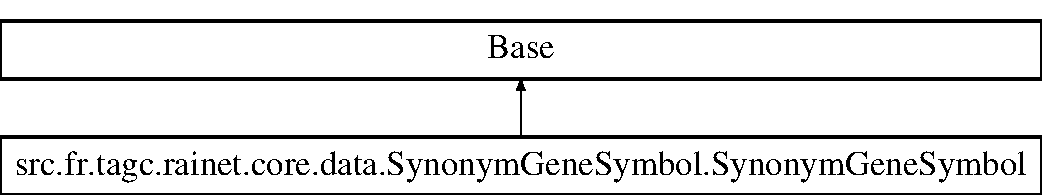
\includegraphics[height=2.000000cm]{classsrc_1_1fr_1_1tagc_1_1rainet_1_1core_1_1data_1_1SynonymGeneSymbol_1_1SynonymGeneSymbol}
\end{center}
\end{figure}
\subsection*{Static Public Attributes}
\begin{DoxyCompactItemize}
\item 
\hypertarget{classsrc_1_1fr_1_1tagc_1_1rainet_1_1core_1_1data_1_1SynonymGeneSymbol_1_1SynonymGeneSymbol_a64069383ae398b9a29700ebfa0716d13}{}tuple {\bfseries id} = Column(Integer, autoincrement=True, primary\+\_\+key=True)\label{classsrc_1_1fr_1_1tagc_1_1rainet_1_1core_1_1data_1_1SynonymGeneSymbol_1_1SynonymGeneSymbol_a64069383ae398b9a29700ebfa0716d13}

\item 
\hypertarget{classsrc_1_1fr_1_1tagc_1_1rainet_1_1core_1_1data_1_1SynonymGeneSymbol_1_1SynonymGeneSymbol_a60b0caa4ff16ab1c362f6dffdfdf2f14}{}tuple {\bfseries protein\+\_\+id} = Column(Integer, Foreign\+Key(\textquotesingle{}Protein.\+uniprot\+A\+C\textquotesingle{}))\label{classsrc_1_1fr_1_1tagc_1_1rainet_1_1core_1_1data_1_1SynonymGeneSymbol_1_1SynonymGeneSymbol_a60b0caa4ff16ab1c362f6dffdfdf2f14}

\item 
\hypertarget{classsrc_1_1fr_1_1tagc_1_1rainet_1_1core_1_1data_1_1SynonymGeneSymbol_1_1SynonymGeneSymbol_a8e3ff826f0c90631c48a98fbec986121}{}tuple {\bfseries uniprot\+Gene\+Symbol} = Column( String)\label{classsrc_1_1fr_1_1tagc_1_1rainet_1_1core_1_1data_1_1SynonymGeneSymbol_1_1SynonymGeneSymbol_a8e3ff826f0c90631c48a98fbec986121}

\end{DoxyCompactItemize}


\subsection{Detailed Description}
This class describe a gene symbol that is a synonym of a main gene symbol of a protein this class has a many-\/to-\/one relationship with the class Protein. 

The documentation for this class was generated from the following file\+:\begin{DoxyCompactItemize}
\item 
src/fr/tagc/rainet/core/data/Synonym\+Gene\+Symbol.\+py\end{DoxyCompactItemize}

\hypertarget{classsrc_1_1fr_1_1tagc_1_1rainet_1_1core_1_1util_1_1parser_1_1TSVParser_1_1TSVParser}{}\section{src.\+fr.\+tagc.\+rainet.\+core.\+util.\+parser.\+T\+S\+V\+Parser.\+T\+S\+V\+Parser Class Reference}
\label{classsrc_1_1fr_1_1tagc_1_1rainet_1_1core_1_1util_1_1parser_1_1TSVParser_1_1TSVParser}\index{src.\+fr.\+tagc.\+rainet.\+core.\+util.\+parser.\+T\+S\+V\+Parser.\+T\+S\+V\+Parser@{src.\+fr.\+tagc.\+rainet.\+core.\+util.\+parser.\+T\+S\+V\+Parser.\+T\+S\+V\+Parser}}


This class is a parser of tab separated text file.  


Inheritance diagram for src.\+fr.\+tagc.\+rainet.\+core.\+util.\+parser.\+T\+S\+V\+Parser.\+T\+S\+V\+Parser\+:\begin{figure}[H]
\begin{center}
\leavevmode
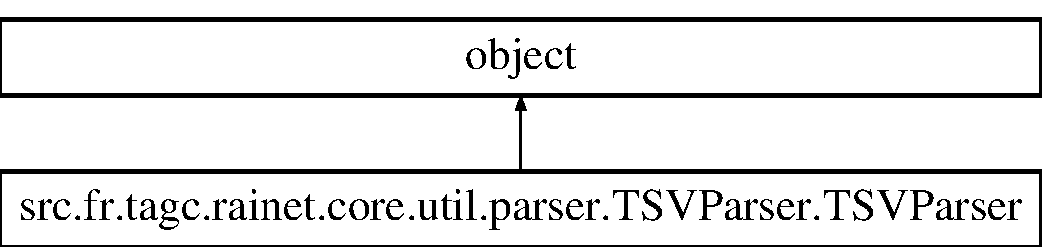
\includegraphics[height=2.000000cm]{classsrc_1_1fr_1_1tagc_1_1rainet_1_1core_1_1util_1_1parser_1_1TSVParser_1_1TSVParser}
\end{center}
\end{figure}
\subsection*{Static Public Member Functions}
\begin{DoxyCompactItemize}
\item 
def \hyperlink{classsrc_1_1fr_1_1tagc_1_1rainet_1_1core_1_1util_1_1parser_1_1TSVParser_1_1TSVParser_a88be88273475e14a025143245a1067c6}{parse\+\_\+file} (file\+\_\+path, has\+\_\+headers, header\+\_\+list, class\+\_\+name, parameter\+\_\+name\+\_\+list, comment\+\_\+symbol)
\begin{DoxyCompactList}\small\item\em This method parses the provided T\+S\+V file, looking for headers if required and creating one Object of the requested Class per line. \end{DoxyCompactList}\end{DoxyCompactItemize}


\subsection{Detailed Description}
This class is a parser of tab separated text file. 

The class contains methods allowing to parse any T\+S\+V file by creating a specific type of Object for each line found The parser have to received as input\+:
\begin{DoxyItemize}
\item The path to the file to parse
\item The information on the presence or not of column headers in the file
\item The ordered list of column headers (if headers are not present or if user want to overwrite file header values)
\item The name of the Class corresponding to Object to be created for each file line
\item The ordered list of header names to use to call the Class constructor
\item The comment symbol 
\end{DoxyItemize}

\subsection{Member Function Documentation}
\hypertarget{classsrc_1_1fr_1_1tagc_1_1rainet_1_1core_1_1util_1_1parser_1_1TSVParser_1_1TSVParser_a88be88273475e14a025143245a1067c6}{}\index{src\+::fr\+::tagc\+::rainet\+::core\+::util\+::parser\+::\+T\+S\+V\+Parser\+::\+T\+S\+V\+Parser@{src\+::fr\+::tagc\+::rainet\+::core\+::util\+::parser\+::\+T\+S\+V\+Parser\+::\+T\+S\+V\+Parser}!parse\+\_\+file@{parse\+\_\+file}}
\index{parse\+\_\+file@{parse\+\_\+file}!src\+::fr\+::tagc\+::rainet\+::core\+::util\+::parser\+::\+T\+S\+V\+Parser\+::\+T\+S\+V\+Parser@{src\+::fr\+::tagc\+::rainet\+::core\+::util\+::parser\+::\+T\+S\+V\+Parser\+::\+T\+S\+V\+Parser}}
\subsubsection[{parse\+\_\+file}]{\setlength{\rightskip}{0pt plus 5cm}def src.\+fr.\+tagc.\+rainet.\+core.\+util.\+parser.\+T\+S\+V\+Parser.\+T\+S\+V\+Parser.\+parse\+\_\+file (
\begin{DoxyParamCaption}
\item[{}]{file\+\_\+path, }
\item[{}]{has\+\_\+headers, }
\item[{}]{header\+\_\+list, }
\item[{}]{class\+\_\+name, }
\item[{}]{parameter\+\_\+name\+\_\+list, }
\item[{}]{comment\+\_\+symbol}
\end{DoxyParamCaption}
)\hspace{0.3cm}{\ttfamily [static]}}\label{classsrc_1_1fr_1_1tagc_1_1rainet_1_1core_1_1util_1_1parser_1_1TSVParser_1_1TSVParser_a88be88273475e14a025143245a1067c6}


This method parses the provided T\+S\+V file, looking for headers if required and creating one Object of the requested Class per line. 


\begin{DoxyParams}{Parameters}
{\em file\+\_\+path} & \+: string -\/ The path to the T\+S\+V file to parse \\
\hline
{\em has\+\_\+header} & \+: boolean -\/ Indicates if the file to parse has a header line \\
\hline
{\em header\+\_\+list} & \+: list$<$string$>$ -\/ Ordered list of headers name (could be None) \\
\hline
{\em class\+\_\+name} & \+: string -\/ name of the class to instantiate \\
\hline
{\em parameter\+\_\+name\+\_\+list} & \+: list$<$string$>$ -\/ Ordered list of parameters used to instantiate the Class \\
\hline
{\em comment\+\_\+symbol} & \+: string -\/ symbol used to comment lines in the file to parse\\
\hline
\end{DoxyParams}
\begin{DoxyReturn}{Returns}
None 
\end{DoxyReturn}


The documentation for this class was generated from the following file\+:\begin{DoxyCompactItemize}
\item 
src/fr/tagc/rainet/core/util/parser/T\+S\+V\+Parser.\+py\end{DoxyCompactItemize}

%--- End generated contents ---

% Index
\backmatter
\newpage
\phantomsection
\clearemptydoublepage
\addcontentsline{toc}{chapter}{Index}
\printindex

\end{document}
